\section*{Datos generales la entidad}

\begin{frame}{Procesos desarrollados durante la práctica}
	\begin{minipage}{0.35\textwidth}
		\begin{figure}[H]
			\captionsetup{width=\textwidth}
			\centering
			
\includegraphics[width=0.5\linewidth]{2.2.pdf}
			\caption[Logotipo de la Municipalidad Distrital de Tamburco]{Logotipo de la Municipalidad Distrital de Tamburco}
			\label{fig:mdt-1}
		\end{figure}
	\end{minipage}
	\quad
	\begin{minipage}{0.55\textwidth}
		\begin{block}{Datos}
			% Table generated by Excel2LaTeX from sheet 'Sheet1'
			\begin{table}[H]
				\centering
				%\caption{Add caption}
				\resizebox{\textwidth}{!}{%
					\begin{tabular}{ll}
						Razón social                   & Municipalidad distrital de Tamburco                  \\
						R.U.C                          & 20175824619                                          \\
						Nombre del representante legal & \multicolumn{1}{l}{Lic. Raúl Silva Campos}           \\
						Nombre del jefe inmediato      & \multicolumn{1}{l}{Ing. Alex Kevin Pumacahua Ccahua} \\
						C.I.P.                         & 302459                                               \\
						Telefono                       & 931677650                                            \\
					\end{tabular}%
				}
				\label{tab:addlabel}%
			\end{table}%  
		\end{block}
	\end{minipage}
\end{frame}
%%%%%%%%%%%%%%%%%%%%%%%%%%%%%%% SLIDE 2 %%%%%%%%%%%%%%%%%%%%%%%%%%%%%%%%%%
%\subsection*{Actividad específica}
\begin{frame}{Organigrama }
    \begin{minipage}{0.45\textwidth}
        \begin{figure}[H]
            \centering
            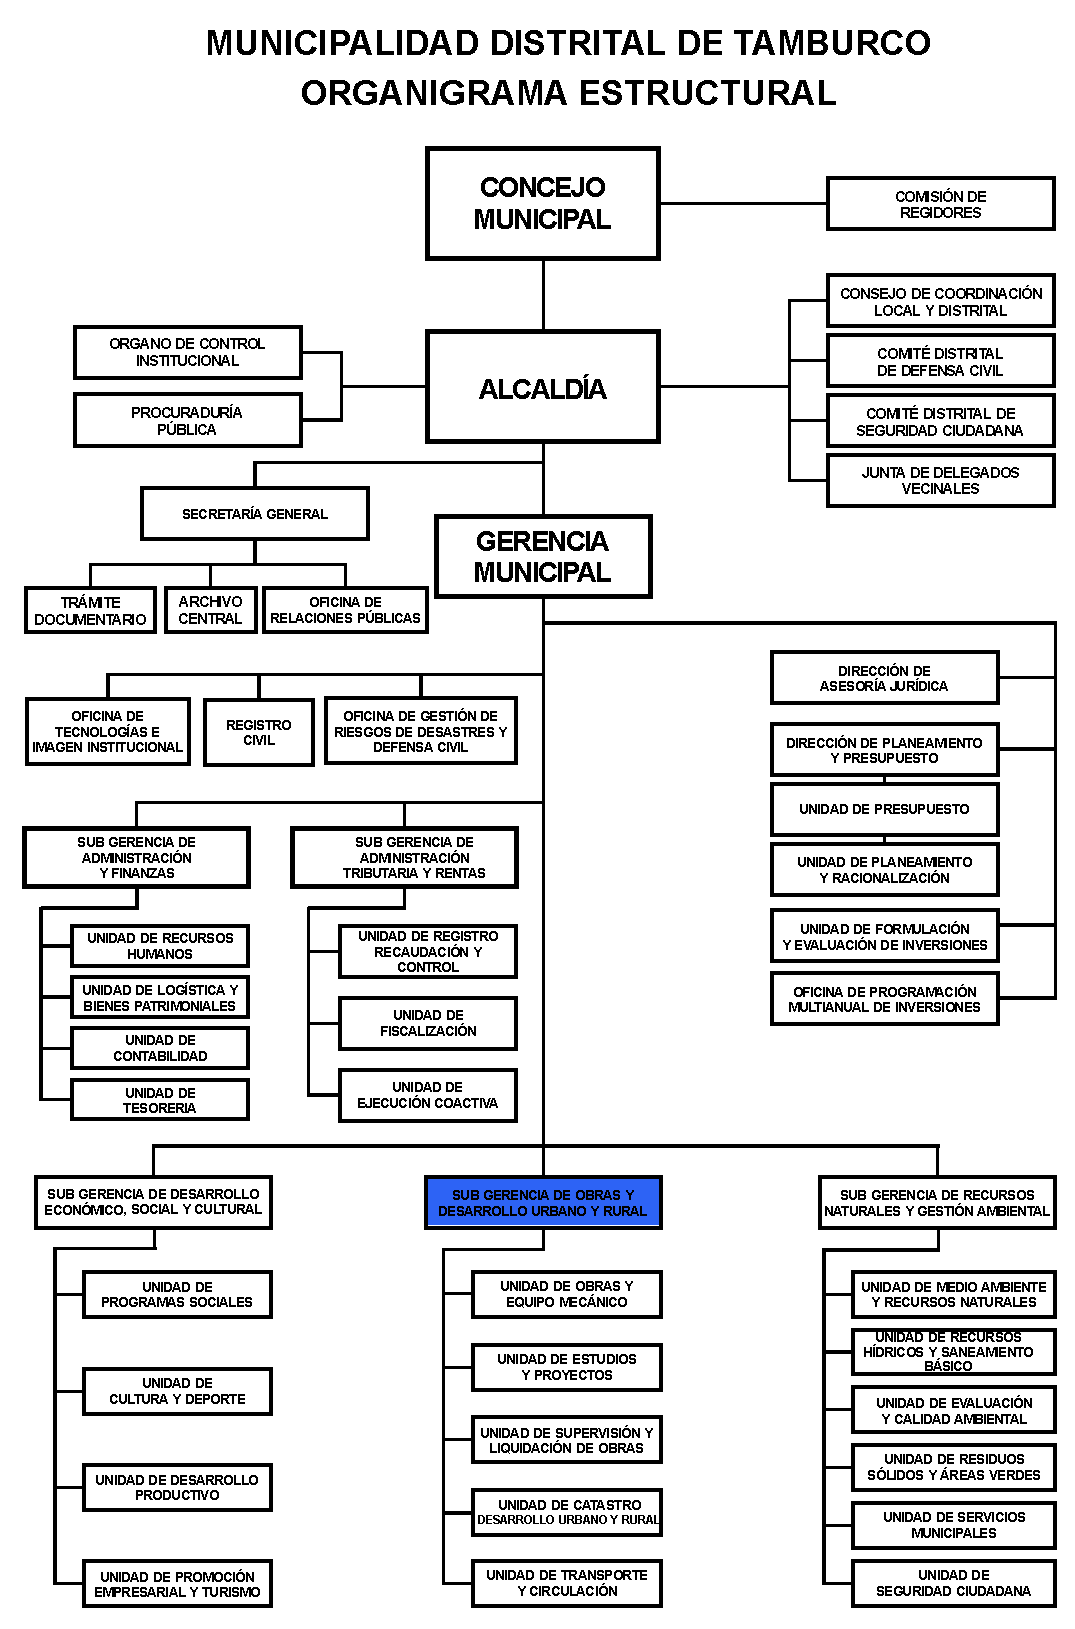
\includegraphics[height=5.5cm]{2.4.pdf}
            \caption[Organigrama de la Municipalidad Distrital de Tamburco]{Fuente:Municipalidad Distrital de Tamburco}
            \label{fig:organigrama-tamburco}
        \end{figure}
    \end{minipage}
    \quad
    \begin{minipage}{0.45\textwidth}
        \begin{figure}[H]
            \captionsetup{width=0.8\textwidth}
            \centering
            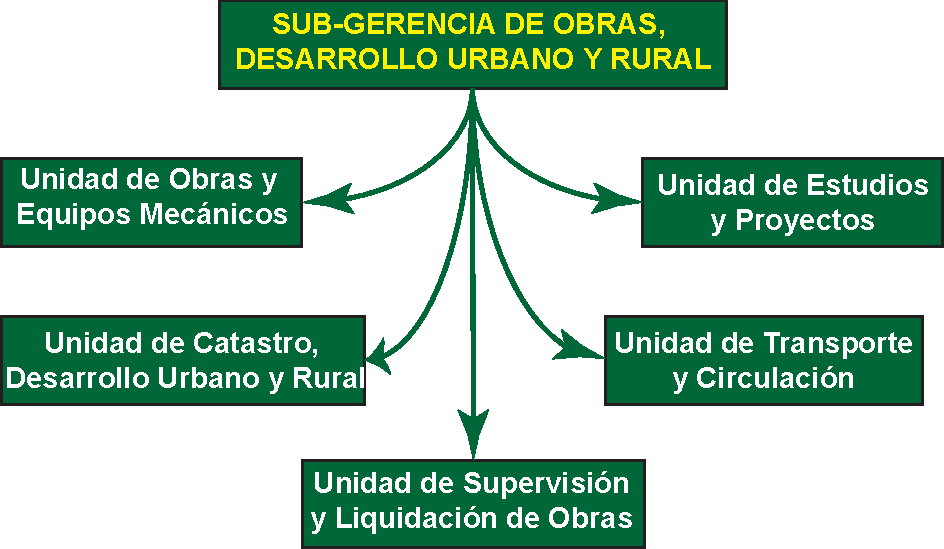
\includegraphics[width=0.8\textwidth]{2.5.pdf}
            \caption{Distribución en unidades de la SGODUR}
            \label{fig:2.5}
        \end{figure}
    \end{minipage}
\end{frame}